\documentclass[11pt]{article}

\usepackage[margin=1in]{geometry}
\usepackage[T1]{fontenc}
\usepackage[utf8]{inputenc}
\usepackage{lmodern}
\usepackage{microtype}
\usepackage{amsmath, amssymb}
\usepackage{booktabs}
\usepackage{xcolor}
\usepackage{hyperref}
\usepackage{enumitem}
\usepackage{listings}
\usepackage{longtable}
\usepackage{graphicx}

\hypersetup{
  colorlinks=true,
  linkcolor=blue!50!black,
  urlcolor=blue!50!black,
  citecolor=blue!50!black
}

\lstset{
  basicstyle=\ttfamily\small,
  keywordstyle=\color{blue!60!black},
  commentstyle=\color{green!40!black},
  stringstyle=\color{red!45!black},
  showstringspaces=false,
  frame=single,
  breaklines=true,
  columns=fullflexible
}

\title{RECAP for Physical Intelligence VLAs:\\A Concept Note and Experimental Snapshot}
\author{Andy Park\\\href{mailto:andypark.purdue@gmail.com}{andypark.purdue@gmail.com}}
\date{April 18, 2026}

\begin{document}
\maketitle

\begin{abstract}
This note captures our current understanding of RECAP---\emph{RL with Experience \& Corrections via Advantage-conditioned Policies}---as used in Physical Intelligence's $\pi^{*}_{0.6}$ system. The core idea is to adapt advantage from reinforcement learning into a form that works naturally for a very large vision-language-action model: estimate advantage offline, binarize it, and feed it back into the policy as a conditioning token. This converts heterogeneous robot data into a stable supervised learning problem while still improving the policy beyond raw imitation. We also summarize the exact iterative training loop, the role of the value function, why the method is particularly well matched to VLAs, and the behavior seen in our local toy experiments.
\end{abstract}

\section{Executive Summary}

The ``advantage'' in RECAP is a VLA-friendly version of the classic RL signal:
\[
A^{\pi}(s, a) = Q^{\pi}(s, a) - V^{\pi}(s).
\]
In ordinary actor-critic RL, this quantity drives policy-gradient updates. In RECAP, the same concept is used differently. Instead of backpropagating policy gradients through a giant generative action model, the system:
\begin{enumerate}[leftmargin=1.5em]
  \item trains a smaller value model to predict future return,
  \item computes an estimated advantage for each action in the dataset,
  \item binarizes that estimate into a positive/negative indicator,
  \item conditions the VLA on that indicator during supervised action training, and
  \item requests \emph{positive-advantage} behavior at inference time.
\end{enumerate}

This is the central reason RECAP is compelling for Physical Intelligence style systems. It allows a large VLA to learn from all available robot experience---good demonstrations, mixed autonomous rollouts, and explicit human corrections---without depending on PPO-style optimization on the full model.

\section{Advantage from First Principles}

\subsection{Standard RL Refresher}

The value function measures expected future return from a state:
\[
V^{\pi}(s) = \mathbb{E}\!\left[\sum_{t=0}^{T} r_t \,\middle|\, s_0 = s, \pi \right].
\]
The state-action value function measures expected return from taking a specific action first:
\[
Q^{\pi}(s, a) = \mathbb{E}\!\left[\sum_{t=0}^{T} r_t \,\middle|\, s_0 = s, a_0 = a, \pi \right].
\]
Their difference is the advantage:
\[
A^{\pi}(s, a) = Q^{\pi}(s, a) - V^{\pi}(s).
\]

Intuitively:
\begin{itemize}[leftmargin=1.5em]
  \item if \(A^{\pi}(s, a) > 0\), the action did better than the policy's baseline expectation at that state;
  \item if \(A^{\pi}(s, a) < 0\), the action was worse than expected.
\end{itemize}

In locomotion RL or simulated control, this signal is often used directly inside online actor-critic methods such as PPO. For a 5B-parameter VLA with a complex generative action head, that route is much less attractive. RECAP keeps the credit-assignment value of advantage while avoiding direct policy-gradient updates on the full model.

\subsection{RECAP's Key Shift}

RECAP turns advantage into \emph{conditioning information}. Instead of asking the VLA to optimize a large RL objective directly, it asks the model to answer a simpler supervised question:

\begin{quote}
``Given the observation, language command, and a token that says whether this action had positive or negative advantage, what action should be generated?''
\end{quote}

That shift is what makes the algorithm fit the VLA setting.

\section{RECAP Mechanics}

\subsection{Task-Agnostic Reward}

RECAP uses a simple sparse reward:
\[
r_t =
\begin{cases}
0 & \text{if the episode ends in success} \\
-C_{\text{fail}} & \text{if the episode ends in failure} \\
-1 & \text{otherwise.}
\end{cases}
\]

The values are normalized per task to \((-1, 0]\), so \(0\) corresponds to a perfect outcome and more negative values correspond to slower or failed executions. The reward is intentionally generic: finish quickly and do not fail.

\subsection{Value Function}

A smaller critic predicts expected return from the current observation \(o_t\) and language instruction \(\ell\). In the \(\pi^{*}_{0.6}\) setup, this is a much smaller vision-language model than the action model itself. It is trained distributionally over binned return targets:
\[
\min_{\phi}\; \mathbb{E}_{\tau} \left[\sum_t H\!\left(R_t^B(\tau),\; p_{\phi}(V \mid o_t, \ell)\right)\right].
\]

The useful intuition is that the value function acts like a progress estimator or ``GPS.'' It learns whether the robot is on a trajectory that still looks recoverable and productive, or whether it has drifted toward failure.

\subsection{Advantage Estimation}

RECAP uses an \(N\)-step bootstrapped advantage estimate:
\[
A^{\pi}(o_t, a_t)
=
\left(\sum_{t'=t}^{t+N-1} r_{t'} + V^{\pi}(o_{t+N})\right)
- V^{\pi}(o_t).
\]

Interpretation:
\begin{itemize}[leftmargin=1.5em]
  \item the first term is the realized short-horizon future after taking the action,
  \item the second term is the baseline expectation before the action.
\end{itemize}

If the robot made unusually good progress, the advantage is positive. If the action made future success less likely, the advantage is negative.

\subsection{Binarization}

Rather than feeding a noisy scalar advantage value into the policy, RECAP thresholds it:
\[
I_t = \mathbb{1}\{A(o_t, a_t) > \epsilon_{\ell}\}.
\]

This gives a simple binary label:
\begin{itemize}[leftmargin=1.5em]
  \item \texttt{Advantage: positive}
  \item \texttt{Advantage: negative}
\end{itemize}

Task-specific thresholds are used so that the positive set has a controlled frequency. During fine-tuning, human correction actions can simply be forced into the positive class.

\subsection{Advantage-Conditioned Policy Training}

The policy is trained with a supervised objective on all data:
\[
\min_{\theta}\; \mathbb{E}\Bigl[
-\log \pi_{\theta}(a_t \mid o_t, \ell)
- \alpha \log \pi_{\theta}(a_t \mid I_t, o_t, \ell)
\Bigr].
\]

The indicator token is randomly dropped some of the time during training. This mirrors classifier-free guidance style conditioning and allows the model to interpolate between unconditional and advantage-conditioned behavior at test time.

At inference, the system simply requests \emph{positive-advantage} behavior. In effect, the policy is nudged toward actions that look more like the high-quality portion of the dataset, even though the model was trained on a broad mixture of behavior.

\section{Exact Iterative RECAP Loop}

The algorithm can be viewed as an iterative offline RL loop wrapped around a VLA:
\begin{align*}
&\text{Require: multi-task demonstration dataset } \mathcal{D}_{\text{demo}} \\
&1:\ \text{Train } V_{\text{pre}} \text{ on } \mathcal{D}_{\text{demo}} \\
&2:\ \text{Train } \pi_{\text{pre}} \text{ on } \mathcal{D}_{\text{demo}} \text{ with advantage conditioning} \\
&3:\ \text{Initialize task dataset } \mathcal{D}_{\ell} \\
&4:\ \text{Train } V_{\ell}^{0} \text{ from } V_{\text{pre}} \text{ on } \mathcal{D}_{\ell} \\
&5:\ \text{Train } \pi_{\ell}^{0} \text{ from } \pi_{\text{pre}} \text{ on } \mathcal{D}_{\ell} \\
&6:\ \textbf{for } k = 1 \textbf{ to } K \textbf{ do} \\
&7:\ \quad \text{Collect autonomous rollouts and optional human corrections with } \pi_{\ell}^{k-1} \\
&8:\ \quad \text{Add the new data to } \mathcal{D}_{\ell} \\
&9:\ \quad \text{Train } V_{\ell}^{k} \text{ from } V_{\text{pre}} \text{ on updated } \mathcal{D}_{\ell} \\
&10:\ \quad \text{Train } \pi_{\ell}^{k} \text{ from } \pi_{\text{pre}} \text{ on updated } \mathcal{D}_{\ell} \\
&11:\ \textbf{end for.}
\end{align*}

Two design choices matter:
\begin{itemize}[leftmargin=1.5em]
  \item The critic is always reinitialized from the pre-trained value model rather than only warm-started from the previous task critic.
  \item The policy is always fine-tuned from the pre-trained VLA rather than recursively fine-tuned from the latest on-robot checkpoint.
\end{itemize}

This keeps the system anchored to the generalist prior while still allowing iterative specialization.

\section{Why the Value Function Visualization Matters}

The value plots shown in the blog and paper are among the best intuition-building tools for RECAP.

For successful episodes:
\begin{itemize}[leftmargin=1.5em]
  \item the value rises as the robot completes the meaningful subgoals of the task,
  \item temporary plateaus often correspond to transport or repositioning,
  \item small dips can reflect recoverable mistakes such as a slightly bad alignment or grip.
\end{itemize}

For unsuccessful episodes:
\begin{itemize}[leftmargin=1.5em]
  \item the value often drops at the exact moment the task becomes difficult or impossible to recover,
  \item the drop can occur well before the terminal failure label,
  \item this is what enables long-horizon credit assignment in practical robot tasks.
\end{itemize}

The important idea is not just that the value predicts eventual success. It identifies \emph{where progress was created or destroyed} inside a long trajectory. That is the signal the advantage estimate turns into action-level supervision.

\section{Why RECAP Fits VLAs Better Than Classical Online RL}

RECAP is particularly well matched to the Physical Intelligence setting for several reasons:
\begin{enumerate}[leftmargin=1.5em]
  \item \textbf{Heterogeneous data becomes usable.} Demonstrations, autonomous rollouts, and corrections all live in one dataset. The difference is not in whether the data is kept, but in how each action is labeled.
  \item \textbf{Long-horizon manipulation gets credit assignment.} A bad grasp early in a long task can receive a negative signal even if the failure occurs much later.
  \item \textbf{Training remains stable for giant generative policies.} The method preserves supervised learning structure instead of relying on high-variance RL updates on the full VLA.
  \item \textbf{It supports iterative practice.} The robot can deploy, fail, collect corrections, and improve again using the same loop.
\end{enumerate}

This is very different from a typical locomotion setup:
\begin{itemize}[leftmargin=1.5em]
  \item locomotion often uses dense hand-designed reward terms,
  \item optimization is online and actor-critic driven,
  \item the policy may be small enough that PPO-like updates are routine.
\end{itemize}

RECAP instead uses offline or batched relabeling of behavior data and a conditioned policy model.

\section{Toy Interpretation of the Conditioning Trick}

The simplest way to understand the method is:
\begin{enumerate}[leftmargin=1.5em]
  \item train on both good and bad behavior,
  \item tag each action with whether it had positive or negative advantage,
  \item ask for positive behavior at inference time.
\end{enumerate}

The following sketch captures that idea in minimal form:

\begin{lstlisting}[language=Python, caption={Tiny toy sketch of the RECAP conditioning idea.}]
import torch
import torch.nn as nn
import torch.nn.functional as F

class ToyPolicy(nn.Module):
    def __init__(self):
        super().__init__()
        self.fc = nn.Linear(3 + 1, 2)

    def forward(self, state, adv_token):
        x = torch.cat([state, adv_token.unsqueeze(1)], dim=1)
        return self.fc(x)

def generate_data(n=1000):
    states = torch.eye(3)[torch.randint(0, 3, (n,))]
    actions = torch.randint(0, 2, (n,))
    true_good = (torch.rand(n) < 0.8).float()
    advantages = (actions == 1).float() * true_good * 2 - 1
    adv_tokens = (advantages > 0).float()
    return states, actions, adv_tokens

policy = ToyPolicy()
opt = torch.optim.Adam(policy.parameters(), lr=1e-2)
states, actions, adv_tokens = generate_data(5000)

for epoch in range(200):
    logits = policy(states, adv_tokens)
    loss_cond = F.cross_entropy(logits, actions)
    if torch.rand(1) < 0.3:
        logits_uncond = policy(states, torch.zeros_like(adv_tokens))
        loss = loss_cond + F.cross_entropy(logits_uncond, actions)
    else:
        loss = loss_cond
    opt.zero_grad()
    loss.backward()
    opt.step()

with torch.no_grad():
    test_states = torch.eye(3)
    pos_token = torch.ones(3)
    probs = F.softmax(policy(test_states, pos_token), dim=1)
    print(probs[:, 1])
\end{lstlisting}

The point of the toy code is not fidelity to the full VLA stack. It is to show the structural move:
\[
\text{mixed data} \quad + \quad \text{advantage label} \quad \Longrightarrow \quad \text{better policy by conditioning.}
\]

\section{Local Experimental Snapshot}

To ground the concept, we built two toy examples in \texttt{recap\_pi}:
\begin{itemize}[leftmargin=1.5em]
  \item a 2D double-integrator obstacle-navigation task,
  \item a 3D ``drone heist'' task with three ordered objectives: collect artifact, activate uplink, then extract.
\end{itemize}

These are not faithful reproductions of \(\pi^{*}_{0.6}\). They are small experiments designed to expose the exact mode-conflict RECAP is meant to resolve: the model is trained on a mixture of good and bad behavior, while the conditioned variant is prompted toward the high-advantage slice of that data.

\subsection{Results Table}

\begin{center}
\begin{longtable}{@{}llll@{}}
\toprule
\textbf{Experiment} & \textbf{Metric} & \textbf{Plain Imitation} & \textbf{RECAP Conditioned} \\
\midrule
\endhead
2D obstacle navigation & Avg.\ effective steps & 190 & 41 \\
2D obstacle navigation & Success rate & 17\% & 100\% \\
2D obstacle navigation & Collision rate & 83\% & 0\% \\
2D obstacle navigation & Relative success gain & 1.0x baseline & 6.0x higher \\
\midrule
3D drone heist & Avg.\ effective steps & 222 & 111 \\
3D drone heist & Success rate & 19\% & 74\% \\
3D drone heist & Artifact completion & 55\% & 100\% \\
3D drone heist & Uplink activation & 24\% & 74\% \\
3D drone heist & Collision rate & 79\% & 19\% \\
3D drone heist & Relative success gain & 1.0x baseline & 3.88x higher \\
\bottomrule
\end{longtable}
\end{center}

\subsection{Interpretation}

The 2D task demonstrates the cleanest form of the effect. Plain behavior cloning often learns an averaged policy over conflicting trajectories and crashes early, while the conditioned policy consistently takes the successful detour.

The 3D task is more interesting because it has an explicit multi-stage structure. The policy must:
\begin{enumerate}[leftmargin=1.5em]
  \item obtain the artifact,
  \item climb and route toward the uplink,
  \item finish by reaching the extraction zone.
\end{enumerate}

The conditioned policy does not merely improve raw path smoothness. It is much better at preserving task \emph{sequence structure}. In other words, it is more likely to complete the right subgoals in the right order, which is exactly the type of long-horizon behavioral organization RECAP is designed to help with.

\section{Figures and What They Show}

\subsection{2D Comparison Figure}

\begin{figure}[ht]
  \centering
  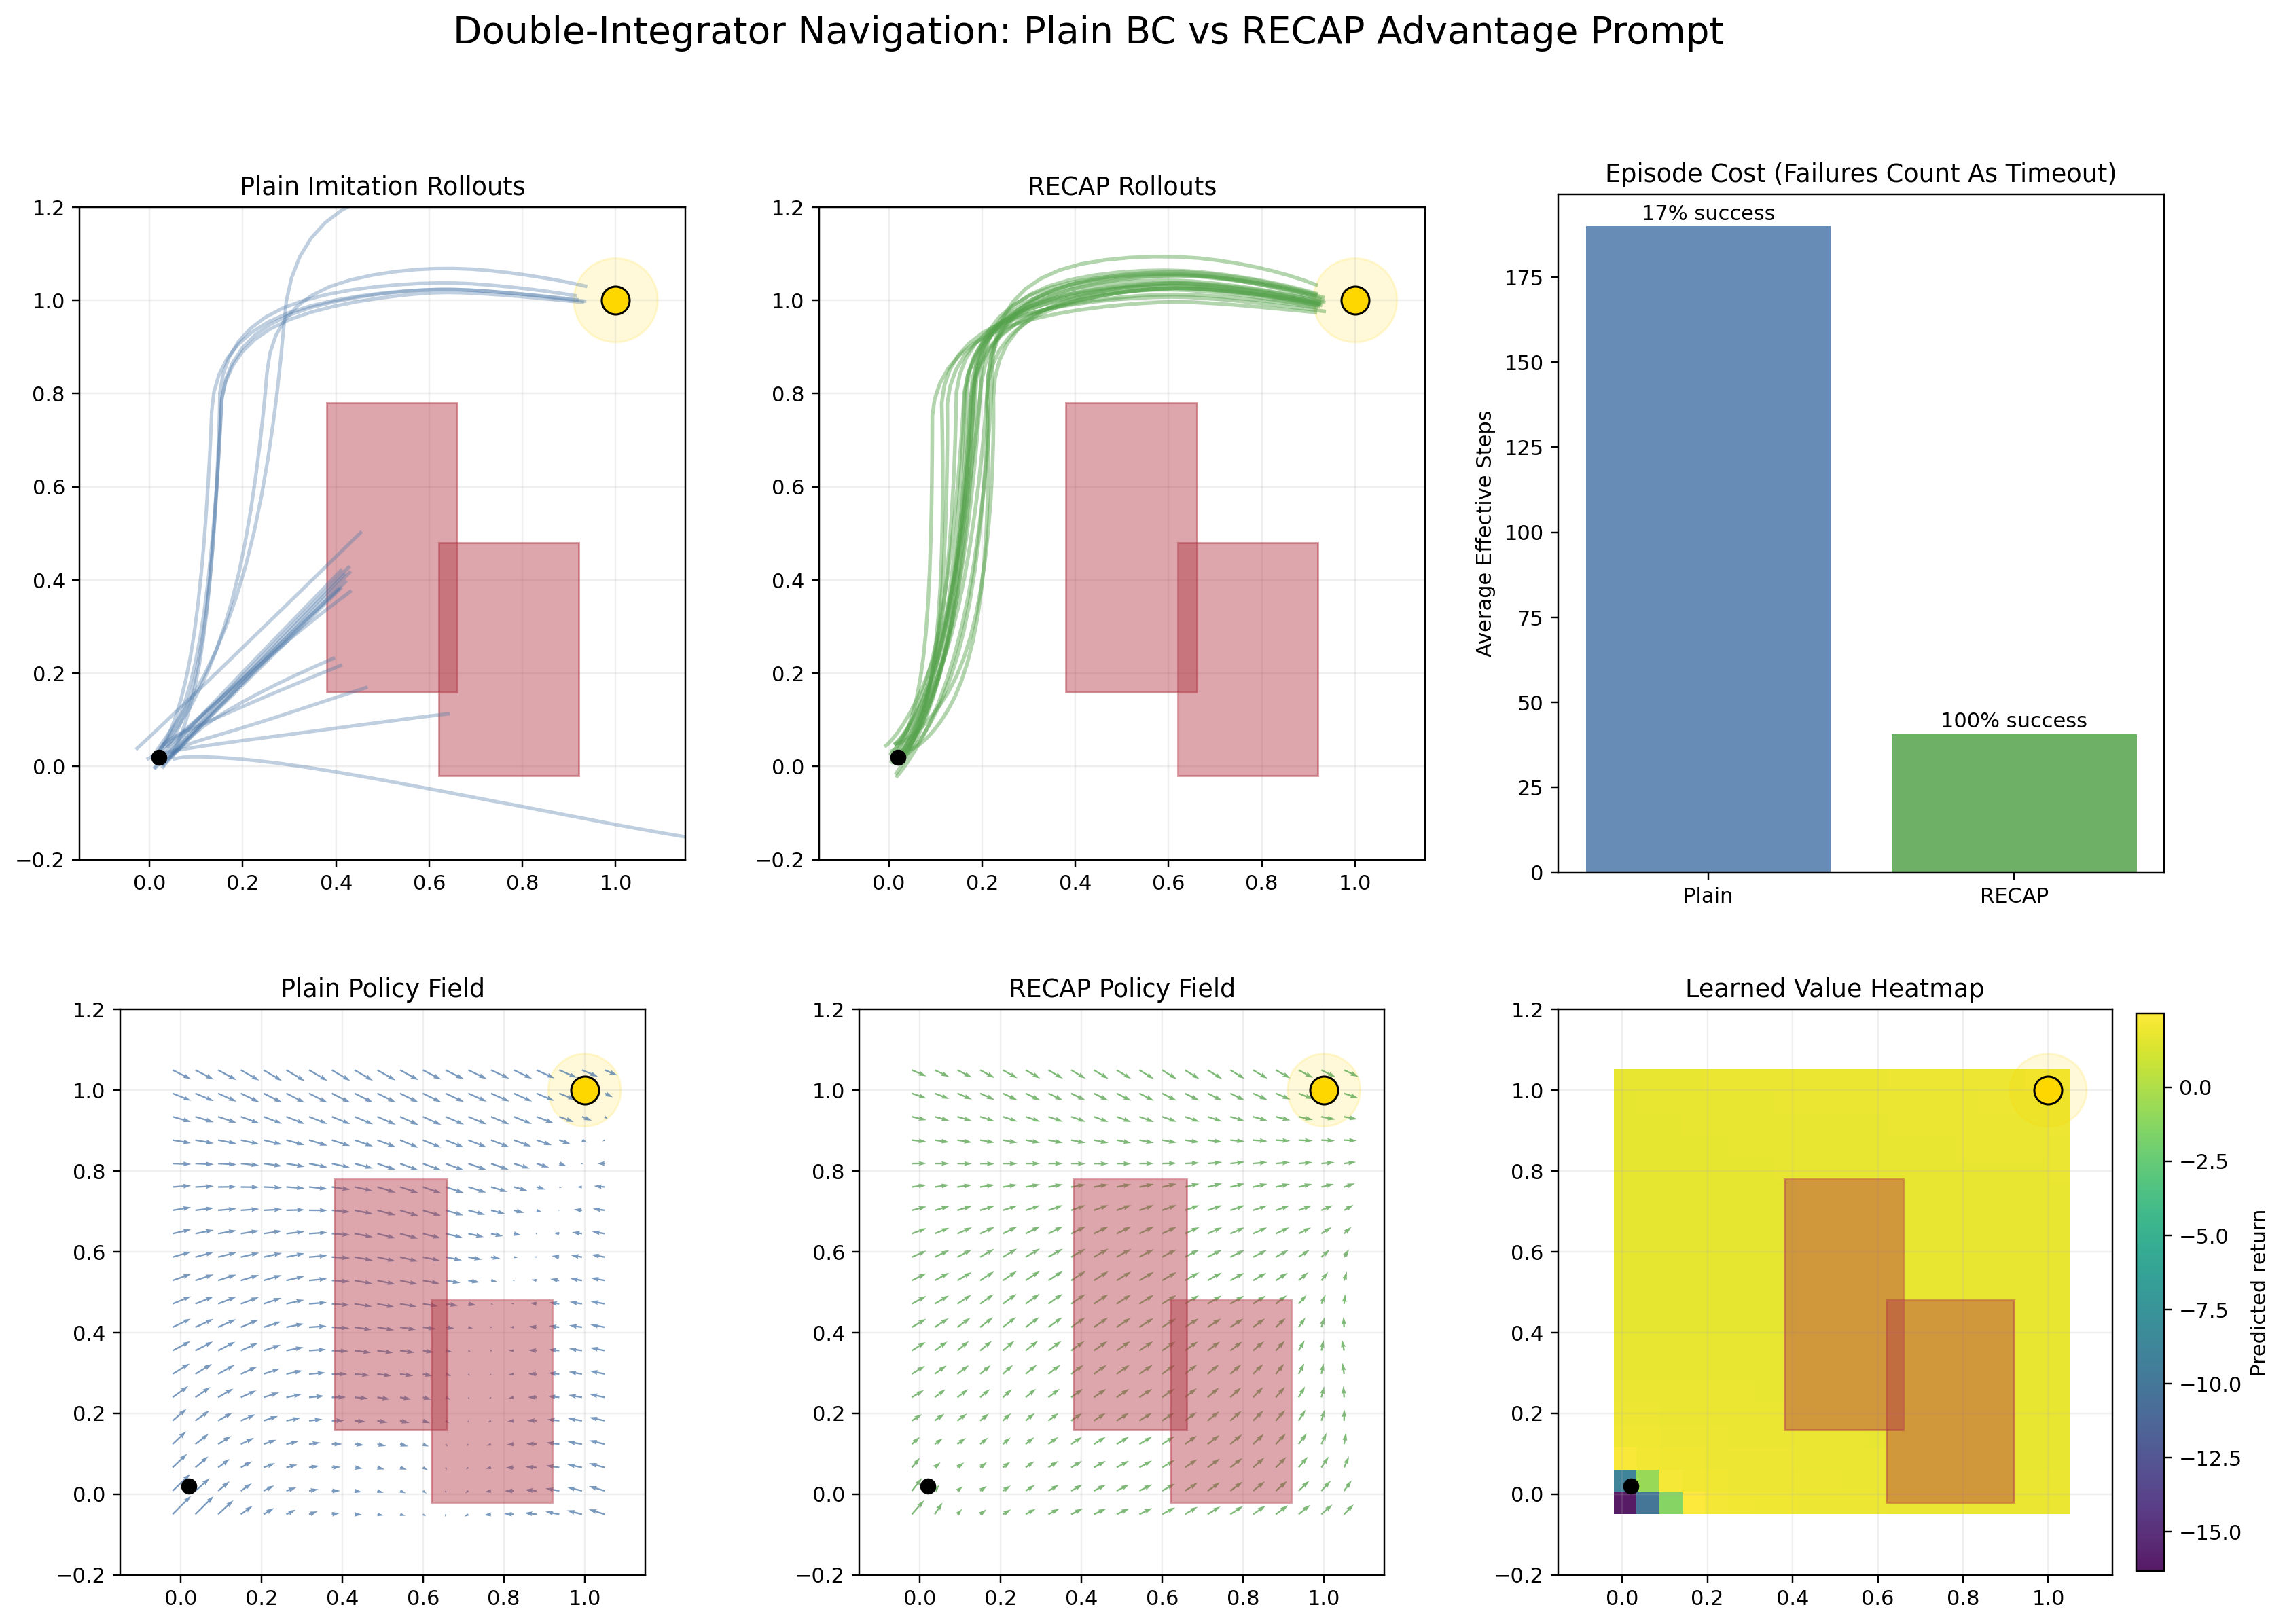
\includegraphics[width=\textwidth]{../outputs/complex_comparison.png}
  \caption{2D obstacle-navigation comparison plot generated by the local toy experiment.}
  \label{fig:2d-comparison}
\end{figure}

Figure~\ref{fig:2d-comparison} is the clearest visual summary of the 2D toy result.
It contains three conceptually important views:
\begin{enumerate}[leftmargin=1.5em]
  \item \textbf{Trajectory overlays.} The plain behavior-cloned rollouts spread into the obstacle region and terminate quickly, which reflects the classic failure mode of averaging across incompatible behaviors. The RECAP-conditioned rollouts instead cluster around the clean successful corridor.
  \item \textbf{Policy field slices.} The quiver plots show that the conditioned policy has learned a more coherent global action field around the obstacle structure, while the plain policy retains ambiguous or self-defeating local directions near the blocked route.
  \item \textbf{Value heatmap and step-cost bars.} These panels show the mechanism behind the improvement. The value estimate assigns higher return to states that belong to the successful detour, and the timeout-penalized step metric confirms that the conditioned policy is not merely ``failing faster'' but actually solving the task.
\end{enumerate}

This figure illustrates the core RECAP idea in its simplest form: once mixed data is relabeled by advantage, the policy can be conditioned toward the successful mode rather than averaging across both success and failure.

\subsection{2D Rollout Stills}

\begin{figure}[ht]
  \centering
  \begin{minipage}[t]{0.48\textwidth}
    \centering
    \includegraphics[width=\textwidth]{figures/plain_rollouts_frame.png}
    \caption*{Plain imitation rollout frame}
  \end{minipage}
  \hfill
  \begin{minipage}[t]{0.48\textwidth}
    \centering
    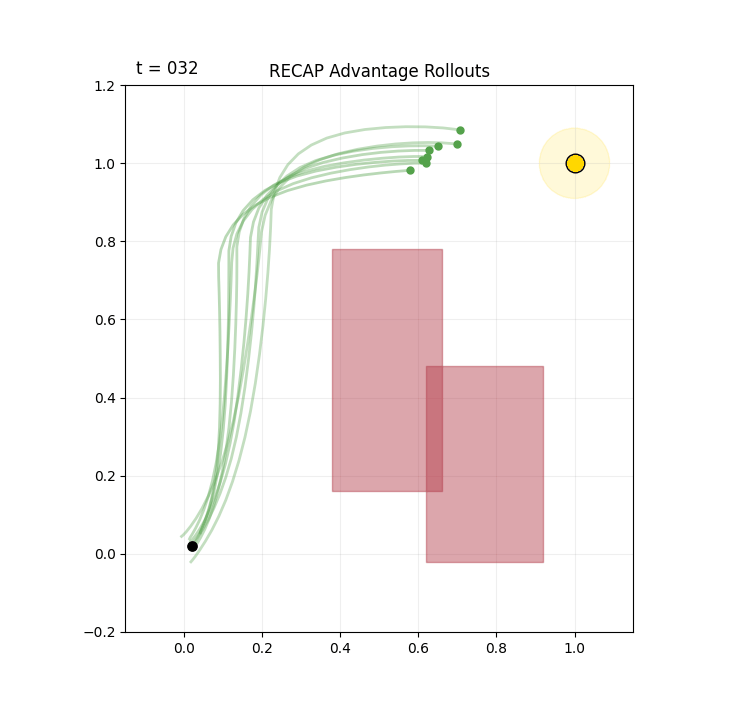
\includegraphics[width=\textwidth]{figures/recap_rollouts_frame.png}
    \caption*{RECAP-conditioned rollout frame}
  \end{minipage}
  \caption{Representative still frames extracted from the 2D rollout GIFs.}
  \label{fig:2d-rollout-stills}
\end{figure}

Figure~\ref{fig:2d-rollout-stills} makes the behavioral distinction more concrete. The plain policy frame shows trajectories crowding the dangerous region and dying early. The conditioned frame shows the rollouts staying organized around the same high-value path. Even in a static snapshot, the difference in mode selection is visible.

\subsection{3D Drone-Heist Comparison Figure}

\begin{figure}[p]
  \centering
  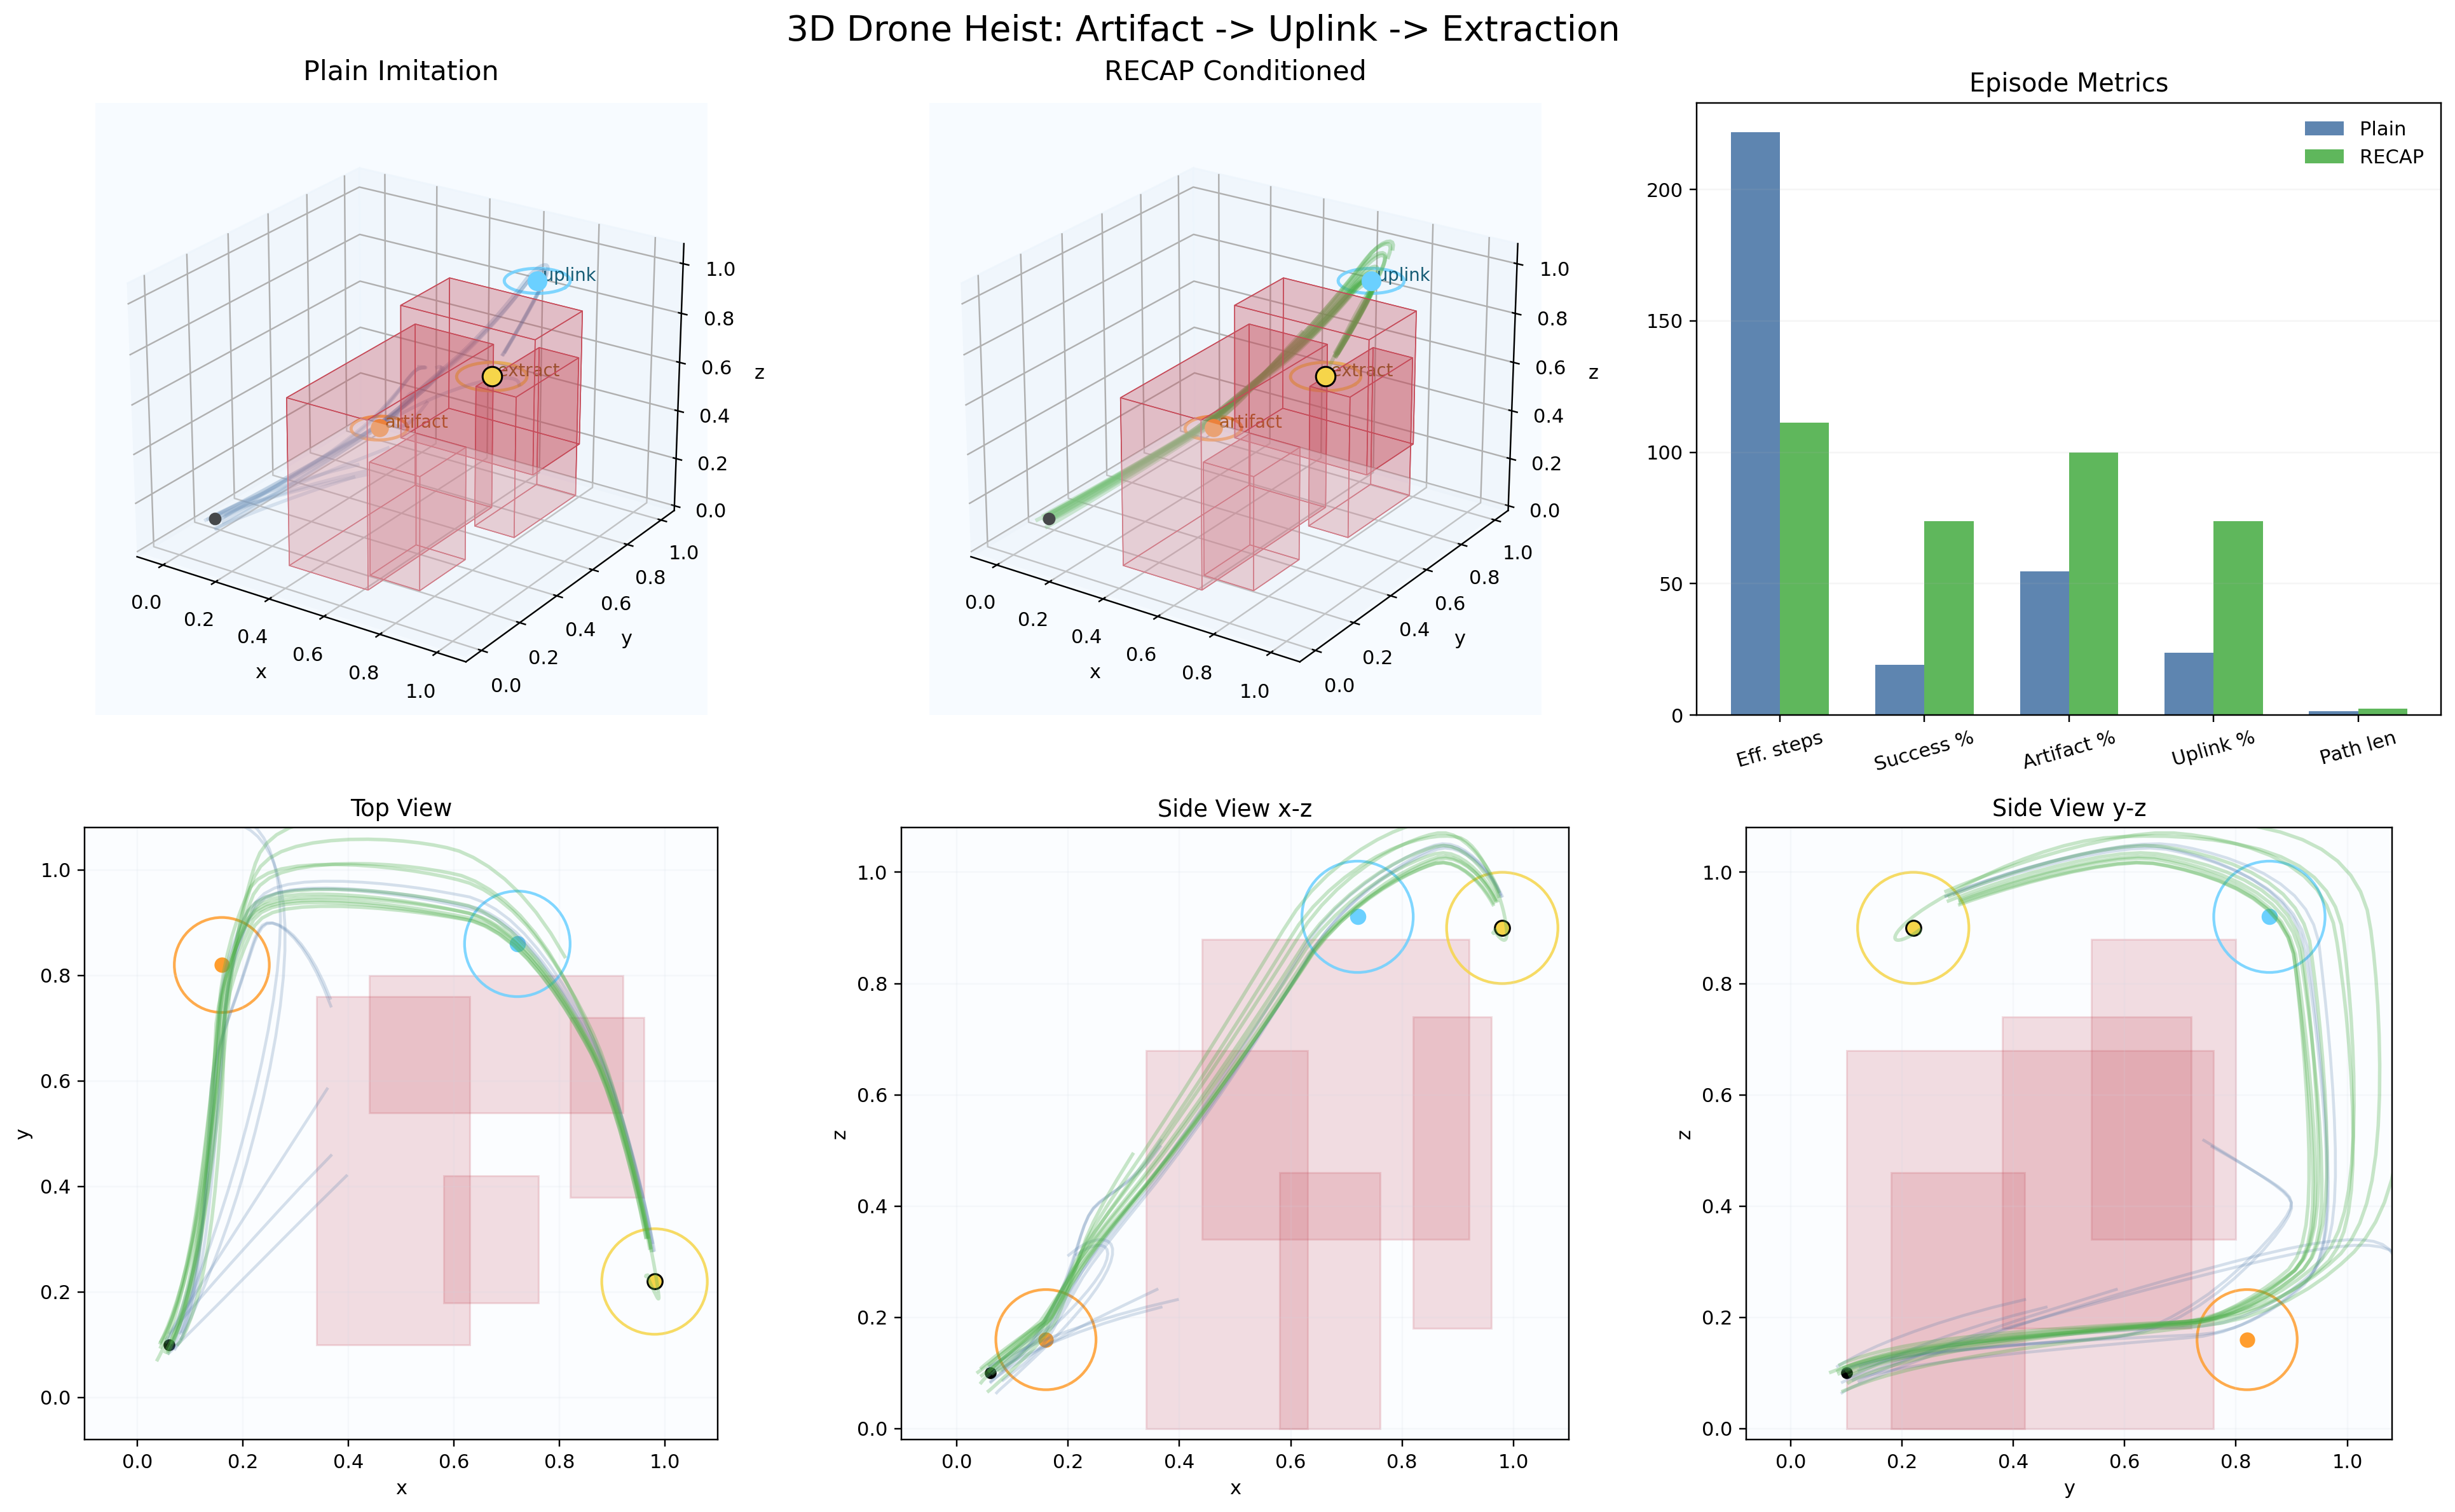
\includegraphics[width=\textwidth]{../outputs/game_3d_comparison.png}
  \caption{3D drone-heist comparison plot generated by the local multi-stage toy experiment.}
  \label{fig:3d-comparison}
\end{figure}

Figure~\ref{fig:3d-comparison} is more interesting because the task has ordered subgoals rather than a single destination. The drone must collect the artifact, activate the uplink, and then extract. The figure is useful in four ways:
\begin{enumerate}[leftmargin=1.5em]
  \item \textbf{3D trajectory panels.} The plain policy often enters blocked geometry after partial progress, whereas the conditioned policy more consistently climbs above the blocking structure and preserves the intended mission sequence.
  \item \textbf{Metric bars.} These show that the gain is not only in success rate. The conditioned policy improves subgoal completion rates as well, especially uplink activation, which is the middle step that depends on the policy maintaining long-horizon structure after obtaining the artifact.
  \item \textbf{Projection views.} The top and side projections reveal why the 3D task is harder. The policy must choose both lateral routing and altitude management. The conditioned policy learns a cleaner high-altitude path through the bottleneck.
  \item \textbf{Narrative meaning.} This figure is the local toy analogue of the RECAP story in the paper: advantage conditioning helps the model choose actions that preserve future solvability, not just immediate motion smoothness.
\end{enumerate}

\subsection{3D Rollout Stills}

\begin{figure}[p]
  \centering
  \begin{minipage}[t]{0.48\textwidth}
    \centering
    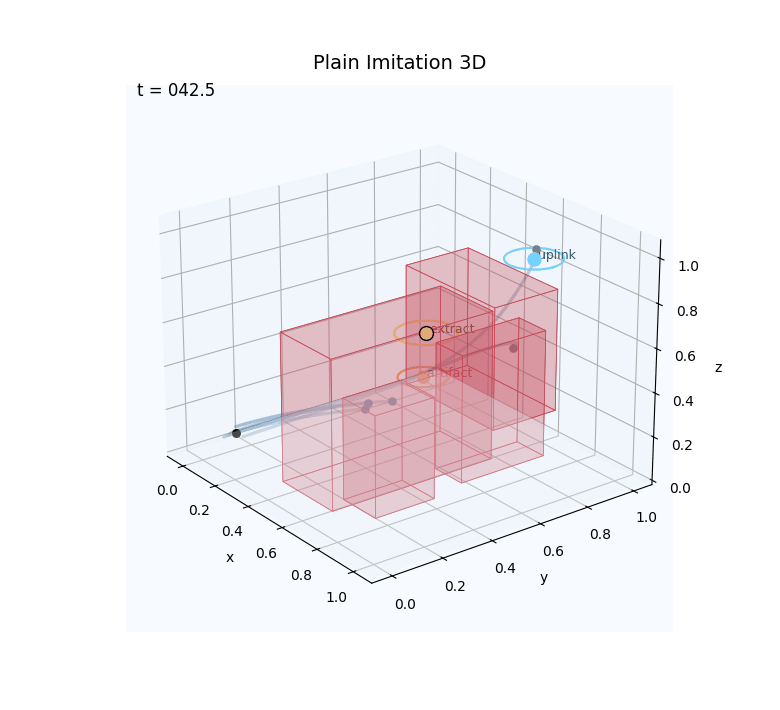
\includegraphics[width=\textwidth]{figures/game_3d_plain_frame.png}
    \caption*{Plain imitation 3D frame}
  \end{minipage}
  \hfill
  \begin{minipage}[t]{0.48\textwidth}
    \centering
    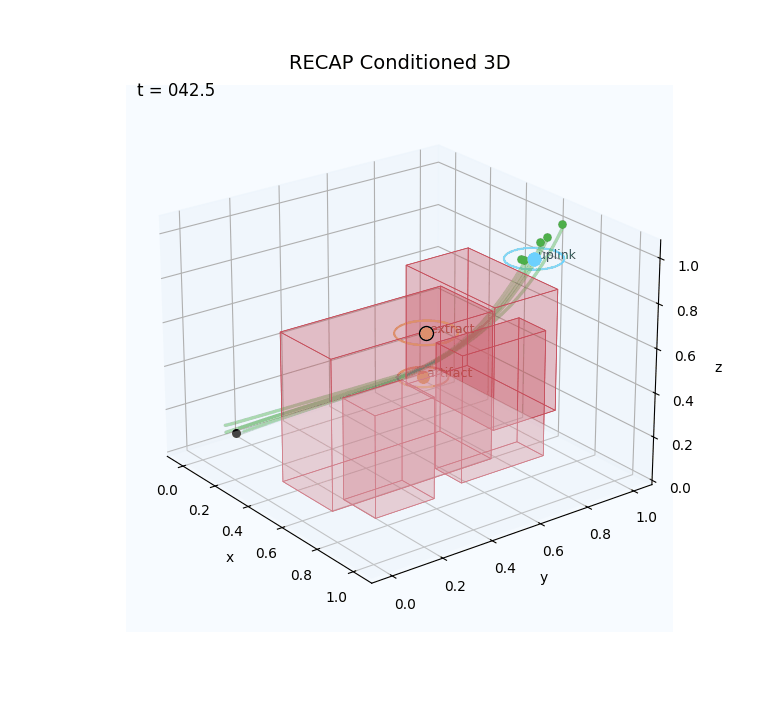
\includegraphics[width=\textwidth]{figures/game_3d_recap_frame.png}
    \caption*{RECAP-conditioned 3D frame}
  \end{minipage}
  \caption{Representative still frames extracted from the 3D GIFs.}
  \label{fig:3d-rollout-stills}
\end{figure}

Figure~\ref{fig:3d-rollout-stills} shows the higher-fidelity 3D animation frames. The plain policy still appears busy and locally competent, but many trajectories are pointed into hazardous regions or poorly aligned with the later subgoals. The conditioned policy frame is visually calmer: the paths are smoother, the altitude choice is more consistent, and the rollouts are better aligned with the extraction corridor after completing the earlier objectives.

The figure is useful because it highlights a subtle but important point. RECAP is not only selecting ``nicer'' actions. It is selecting actions that are better \emph{because they preserve future opportunity}. That is exactly what the advantage label is supposed to encode.

\section{Takeaways}

Our current understanding can be summarized in five points:
\begin{enumerate}[leftmargin=1.5em]
  \item RECAP reuses the semantics of advantage without doing large-scale policy-gradient RL on the main VLA.
  \item The critic provides long-horizon credit assignment in a form compatible with supervised fine-tuning.
  \item Binarization is important because it turns a noisy scalar signal into a robust conditioning token.
  \item Human corrections fit naturally into the same framework by being marked as positive-advantage actions.
  \item The resulting policy can improve over the mixed dataset simply by conditioning on the positive label at inference.
\end{enumerate}

The toy results are consistent with that story. The conditioned policy is not just slightly better calibrated. It is qualitatively better at selecting the successful mode from a mixed behavioral dataset.

\section*{Artifacts}

This writeup accompanies the toy examples in \texttt{recap\_pi}. The current repository also contains rendered comparison plots and GIFs for both the 2D and 3D settings under \texttt{recap\_pi/outputs/}.

\end{document}
